\begin{dang}{Tìm giá trị lớn nhất, giá trị nhỏ nhất của hàm số lượng giác}
	Dựa vào tập giá trị của hàm số lượng giác, chẳng hạn:
	\begin{itemize}
		\item $ -1 \leq \sin x \leq 1 \Rightarrow \left|\begin{aligned}&0 \leq|\sin x| \leq 1\\&0 \leq \sin ^{2} x \leq 1 \end{aligned}\right.$ hoặc $ -1 \leq \cos x \leq 1 \Rightarrow \left|\begin{aligned}&0 \leq|\cos x| \leq 1\\&0 \leq \cos ^{2} x \leq 1. \end{aligned}\right.$
		\item Biến đổi về dạng: $ m \leq y \leq M $.
	\end{itemize}
	Kết luận: $ \max y=M \text { và } \min y=m $.\\
	\textbf{Một số phương pháp tìm GTLN, GTNN}
\begin{enumerate}
	\item Khảo sát parabol: Trong trường hợp hàm số có dạng bậc hai theo một hàm số lượng giác, ta có thể dụng phương pháp đặt ẩn phụ để đưa về hàm bậc hai, sau đó khảo sát hàm này và kết luận.\\			
	\item Sử dụng bất đẳng thức.
	\begin{itemize}
		\item Bất đẳng thức Cauchy:
		\begin{enumEX}[\faCheckCircleO]{1}
			\item $ \forall a, b \geq 0 $ thì $ \dfrac{a+b}{2} \geq \sqrt{a b} $. Dấu \lq\lq =\rq\rq xảy ra khi và chỉ khi $ a=b \geq 0 $.
			\item $ \forall a, b, c \geq 0 $ thì $ \dfrac{a+b+c}{3} \geq \sqrt[3]{a b c} $. Dấu \lq\lq =\rq\rq xảy ra khi và chỉ khi $ a=b=c \geq 0 $.
		\end{enumEX}
		\item Bất đẳng thức Cauchy - Schwarz:
		\begin{enumEX}[\faCheckCircleO]{1}
			\item $ \forall x, y, a, b \in \mathbb{R} $ thì $ |a x+b y| \leq \sqrt{\left(a^{2}+b^{2}\right)\left(x^{2}+y^{2}\right)} $. Dấu \lq\lq =\rq\rq xảy ra khi và chỉ khi $ \dfrac{x}{a}=\dfrac{y}{b} $.
			\item $ \forall x, y \in \mathbb{R}, a, b>0 $ thì $ \dfrac{x^{2}}{a}+\dfrac{y^{2}}{b} \geq \dfrac{(x+y)^{2}}{a+b}$. Dấu \lq\lq =\rq\rq xảy ra khi và chỉ khi $ \dfrac{x}{a}=\dfrac{y}{b} $.
		\end{enumEX}
	\end{itemize}
	\begin{note}
		Trong trường hợp đề bài yêu cầu tìm giá trị lớn nhất và giá trị nhỏ nhất của hàm số lượng giác trên đoạn cho trước, ta sẽ sử dụng đường tròn lượng giác để giới hạn miền của sin hoặc cos. Sau đó thêm bớt giống phương pháp 1 hoặc bậc 2 thì sử dụng parabol.
		\begin{enumEX}[\faCheckCircleO]{2}
			\item $ m \geq f(x), \forall x \in \mathscr{D} \Leftrightarrow m \geq \max\limits_{x \in \mathscr{D}} f(x) $.
			\item $ m \leq f(x), \forall x \in \mathscr{D} \Leftrightarrow m \leq \min\limits_{x \in \mathscr{D}} f(x) $.
		\end{enumEX}
	\end{note}
\end{enumerate}
\end{dang}
\setcounter{bt}{0}% Reset lại số đếm câu hỏi
%Cau1
\begin{bt}%[Ân Trương - DA2]%[1D1B1-1]
	Tìm giá trị lớn nhất và giá trị nhỏ nhất của hàm số $ y=5-3 \cos 4 x $.
	\dapso{$ \max y=8 $ khi $ \cos 4 x=-1 \Leftrightarrow x=\dfrac{\pi}{4}+\dfrac{k\pi}{2}$.
			$ \min y=2 $ khi $ \cos 4 x=1 \Leftrightarrow x=\dfrac{k\pi}{2}$
}
	\loigiai
	{
		Tập xác định: $ \mathscr{D}=\mathbb{R}$. $ \forall x \in \mathbb{R} $, ta có
		\begin{eqnarray*}
			&&-1 \leq \cos 4 x \leq 1 \\
			&\Leftrightarrow& 3 \geq-3 \cos 4 x \geq-3\\
			&\Leftrightarrow& 5+3 \geq 5-3 \cos 4 x \geq 5-3 \\
			&\Leftrightarrow& 2 \leq y \leq 8. 
		\end{eqnarray*}
		\begin{itemize}
			\item $ \max y=8 $ khi $ \cos 4 x=-1 \Leftrightarrow x=\dfrac{\pi}{4}+\dfrac{k\pi}{2}$.
			\item $ \min y=2 $ khi $ \cos 4 x=1 \Leftrightarrow x=\dfrac{k\pi}{2}$
		\end{itemize}
		
	}
\end{bt}
%Cau2
\begin{bt}%[Ân Trương - DA2]%[1D1B1-1]
	Tìm giá trị lớn nhất và giá trị nhỏ nhất của hàm số $ y=2+3 \cos x $.
	\dapso{$ \max y=5 $ khi $ \cos  x=1 \Leftrightarrow x=k2\pi$.
			$ \min y=-1 $ khi $ \cos x=-1 \Leftrightarrow x=\pi +k2\pi$.
}
	\loigiai
	{
		Tập xác định: $ \mathscr{D}=\mathbb{R}$. $ \forall x \in \mathbb{R} $, ta có 
		\begin{eqnarray*}
			&&-1 \leq \cos x \leq 1\\
			&\Leftrightarrow& -3 \geq3 \cos x \geq-3\\
			&\Leftrightarrow&-1 \geq 2+3 \cos  x \geq 5\\
			&\Leftrightarrow& -1 \leq y \leq 5. 
		\end{eqnarray*}
		\begin{itemize}
			\item $ \max y=5 $ khi $ \cos  x=1 \Leftrightarrow x=k2\pi$.
			\item $ \min y=-1 $ khi $ \cos x=-1 \Leftrightarrow x=\pi +k2\pi$.
		\end{itemize}
		
	}
\end{bt}
%Cau3
\begin{bt}%[Ân Trương - DA2]%[1D1B1-1]
	Tìm giá trị lớn nhất và giá trị nhỏ nhất của hàm số $y=3-2 \sin 2 x $.
	\dapso{
		$ \max y=5 $ khi $ \sin 2x=-1 \Leftrightarrow x=-\dfrac{\pi}{4}+k\pi$.
		$ \min y=1 $ khi $ \sin 2x=1 \Leftrightarrow x=\dfrac{\pi}{4}+k\pi$.
	}
	\loigiai
	{
		Tập xác định: $ \mathscr{D}=\mathbb{R}$. $ \forall x \in \mathbb{R} $, ta có 
		\begin{eqnarray*}
			&&-1 \leq \sin 2x \leq 1\\
			&\Leftrightarrow& -2 \leq -2\sin 2x \leq 2\\
			&\Leftrightarrow& 1 \leq 3-2\sin 2x \leq 5\\
			&\Leftrightarrow& 1 \leq y \leq 5.
		\end{eqnarray*}
		\begin{itemize}
			\item $ \max y=5 $ khi $ \sin 2x=-1 \Leftrightarrow x=-\dfrac{\pi}{4}+k\pi$.
			\item $ \min y=1 $ khi $ \sin 2x=1 \Leftrightarrow x=\dfrac{\pi}{4}+k\pi$.
		\end{itemize}
		
	}
\end{bt}
%Cau4
\begin{bt}%[Ân Trương - DA2]%[1D1B1-1]
	Tìm giá trị lớn nhất và giá trị nhỏ nhất của hàm số $ y=3-2|\sin 2 x| $.
	\dapso{
$ \max y=3 $ khi $ \sin 2 x=0 \Leftrightarrow x=\dfrac{k\pi}{2}$.
$ \min y=1$ khi $ \sin 2 x=\pm1 \Leftrightarrow x=\dfrac{\pm\pi}{4}+k\pi$.
	}
	\loigiai
	{
		Tập xác định: $ \mathscr{D}=\mathbb{R}$. $ \forall x \in \mathbb{R} $, ta có 
		\begin{eqnarray*}
			&&0\leq	|\sin 2 x|\leq 1\\
			&\Leftrightarrow&  -2\leq	-2|\sin 2 x|\leq 0\\
			&\Leftrightarrow&  1\leq	3-2|\sin 2 x|\leq 3.
		\end{eqnarray*}
		\begin{itemize}
			\item $ \max y=3 $ khi $ \sin 2 x=0 \Leftrightarrow x=\dfrac{k\pi}{2}$.
			\item $ \min y=1$ khi $ \sin 2 x=\pm1 \Leftrightarrow x=\dfrac{\pm\pi}{4}+k\pi$.
		\end{itemize}
		
	}
\end{bt}
%Cau5
\begin{bt}%[Ân Trương - DA2]%[1D1B1-1]
	Tìm giá trị lớn nhất và giá trị nhỏ nhất của hàm số $ y=\dfrac{1+4 \cos ^{2} x}{3} $.
	\dapso{
$ \max y=\dfrac{5}{3} $ khi $ \cos x=0 \Leftrightarrow x=\dfrac{\pi}{2}+k\pi$.
$ \min y=\dfrac{1}{3} $ khi $ \cos  x=\pm1 \Leftrightarrow x=k\pi$.
	}
	\loigiai
	{
		Tập xác định: $ \mathscr{D}=\mathbb{R}$. $ \forall x \in \mathbb{R} $, ta có 
		\begin{eqnarray*}
			&& 0\leq \cos ^{2} x \leq 1\\
			&\Leftrightarrow& 0\leq 4\cos ^{2} x \leq 4\\
			&\Leftrightarrow& 1\leq 1+4\cos ^{2} x \leq5\\
			&\Leftrightarrow& \dfrac{1}{3}\leq \dfrac{1+4\cos ^{2} x}{3} \leq \dfrac{5}{3}.
		\end{eqnarray*}
		\begin{itemize}
			\item $ \max y=\dfrac{5}{3} $ khi $ \cos x=0 \Leftrightarrow x=\dfrac{\pi}{2}+k\pi$.
			\item $ \min y=\dfrac{1}{3} $ khi $ \cos  x=\pm1 \Leftrightarrow x=k\pi$.
		\end{itemize}
		
	}
\end{bt}
%Cau6
\begin{bt}%[Ân Trương - DA2]%[1D1B1-1]
	Tìm giá trị lớn nhất và giá trị nhỏ nhất của hàm số $ y=1-\dfrac{1}{2} \sin ^{2} 2 x $.
	\dapso{
$ \max y=1 $ khi $ \sin  2 x=0 \Leftrightarrow x=\dfrac{\pi}{4}+\dfrac{k\pi}{2}$.
$ \min y=\dfrac{1}{2} $ khi $ \sin  2 x=\pm1 \Leftrightarrow x=\dfrac{\pi}{4}+\dfrac{k\pi}{2}$.
	}
	\loigiai
	{
		Tập xác định: $ \mathscr{D}=\mathbb{R}$. $ \forall x \in \mathbb{R} $, ta có 
		\begin{eqnarray*}
			&& 0 \leq  \sin ^{2} 2 x \leq 1\\
			&\Leftrightarrow& -\dfrac{1}{2} \leq  -\dfrac{1}{2}\cdot\sin ^{2} 2 x \leq 0\\
			&\Leftrightarrow& \dfrac{1}{2} \leq  -\dfrac{1}{2}\cdot\sin ^{2} 2 x \leq 1.
		\end{eqnarray*}
		\begin{itemize}
			\item $ \max y=1 $ khi $ \sin  2 x=0 \Leftrightarrow x=\dfrac{\pi}{4}+\dfrac{k\pi}{2}$.
			\item $ \min y=\dfrac{1}{2} $ khi $ \sin  2 x=\pm1 \Leftrightarrow x=\dfrac{\pi}{4}+\dfrac{k\pi}{2}$.
		\end{itemize}
		
	}
\end{bt}
%Cau7
\begin{bt}%[Ân Trương - DA2]%[1D1B1-1]
	Tìm giá trị lớn nhất và giá trị nhỏ nhất của hàm số $ y=\sin x+\sin (x+2 \pi / 3) $.
	\dapso{
$ \max y=1 $ khi $ \sin \left (x+\dfrac{\pi}{3}\right )=1 \Leftrightarrow x=\dfrac{\pi}{6}+k2\pi$.
$ \min y=-1 $ khi $ \sin \left (x+\dfrac{\pi}{3}\right )=-1 \Leftrightarrow x=-\dfrac{5\pi}{6}+k2\pi$.
	}
	\loigiai
	{
		Áp dụng công thức \fbox{$ \sin a+\sin b=2 \sin \dfrac{a+b}{2} \cos \dfrac{a-b}{2} $}, ta có
		\begin{equation*}
			y=\sin x + \sin \left (x+\dfrac{2\pi}{3}\right )=-\sin \left (x+\dfrac{\pi}{3}\right ).
		\end{equation*}
		Tập xác định: $ \mathscr{D}=\mathbb{R}$. $ \forall x \in \mathbb{R} $, ta có 
		\begin{equation*}
			-1 \leq -\sin \left (x+\dfrac{\pi}{3}\right ) \leq 1.
		\end{equation*}
		\begin{itemize}
			\item $ \max y=1 $ khi $ \sin \left (x+\dfrac{\pi}{3}\right )=1 \Leftrightarrow x=\dfrac{\pi}{6}+k2\pi$.
			\item $ \min y=-1 $ khi $ \sin \left (x+\dfrac{\pi}{3}\right )=-1 \Leftrightarrow x=-\dfrac{5\pi}{6}+k2\pi$.
		\end{itemize}
		
	}
\end{bt}
%Cau8
\begin{bt}%[Ân Trương - DA2]%[1D1B1-1]
	Tìm giá trị lớn nhất và giá trị nhỏ nhất của hàm số $ y=\cos x+\cos (x+\pi / 3) $.
	\dapso{
$ \max y=\sqrt{3} $ khi $ \cos \left (x+\dfrac{\pi}{6}\right ) =1 \Leftrightarrow x=-\dfrac{\pi}{6}+k2\pi$.
$ \min y=-\sqrt{3} $ khi $ \cos \left (x+\dfrac{\pi}{6}\right )=-1 \Leftrightarrow x=\dfrac{5\pi}{6}+k2\pi$.
	}
	\loigiai
	{
		Áp dụng công thức \fbox{$ \cos a+\cos b=2 \cos \dfrac{a+b}{2} \cos \dfrac{a-b}{2} $}, ta có
		\begin{equation*}
			y=\cos x+\cos \left (x+\dfrac{\pi}{3}\right )=\sqrt{3}\cos \left (x+\dfrac{\pi}{6}\right ).
		\end{equation*}
		Tập xác định: $ \mathscr{D}=\mathbb{R}$. $ \forall x \in \mathbb{R} $, ta có
		\begin{eqnarray*}
			&&-1 \leq \cos \left (x+\dfrac{\pi}{6}\right ) \leq 1\\
			&\Leftrightarrow&  -\sqrt{3} \leq \sqrt{3}\cos \left (x+\dfrac{\pi}{6}\right ) \leq \sqrt{3}.
		\end{eqnarray*} 
		\begin{itemize}
			\item $ \max y=\sqrt{3} $ khi $ \cos \left (x+\dfrac{\pi}{6}\right ) =1 \Leftrightarrow x=-\dfrac{\pi}{6}+k2\pi$.
			\item $ \min y=-\sqrt{3} $ khi $ \cos \left (x+\dfrac{\pi}{6}\right )=-1 \Leftrightarrow x=\dfrac{5\pi}{6}+k2\pi$.
		\end{itemize}
		
	}
\end{bt}


%%%%% Thầy Son Nguyen Truong %%%%%%%%



%%%%%%% Thầy Bùi Thanh Cương %%%%%%%%
\setcounter{bt}{8}
\begin{bt}%[Bùi Thanh Cương-TeX11-Lbt-DuAn2.1]%[1D1K1-5]
	Tìm giá trị lớn nhất và giá trị nhỏ nhất của hàm số $y=\dfrac{4}{2-\sin x}$.
	\dapso{
		$\max\limits_{x \in \mathbb{R}} y=4$ khi $x=\dfrac{\pi}{2}$ và $\min\limits_{x \in \mathbb{R}} y=\dfrac{4}{3}$ khi $x=-\dfrac{\pi}{2}$.
	}
	\loigiai
	{Tập xác định $\mathscr{D}=\mathbb{R}$.\\
		Với mọi $x\in \mathbb{R}$ ta có
		\allowdisplaybreaks
		\begin{eqnarray*}
			& & -1\leq \sin x\leq 1\\
			&\Leftrightarrow& -1\leq -\sin x\leq 1\\
			&\Leftrightarrow&1\leq 2-\sin x\leq 3\\
			&\Leftrightarrow& \dfrac{1}{3}\leq \dfrac{1}{2-\sin x}\leq 1\\
			&\Leftrightarrow& \dfrac{4}{3}\leq \dfrac{4}{2-\sin x}\leq 4.
		\end{eqnarray*} 
		Vậy $\max\limits_{x \in \mathbb{R}} y=4$ khi $x=\dfrac{\pi}{2}$ và $\min\limits_{x \in \mathbb{R}} y=\dfrac{4}{3}$ khi $x=-\dfrac{\pi}{2}$.
	}
\end{bt}
\begin{bt}%[Bùi Thanh Cương-TeX11-Lbt-DuAn2.1]%[1D1K1-5]
	Tìm giá trị lớn nhất và giá trị nhỏ nhất của hàm số $y=\dfrac{8}{3-\cos ^{2} x}$.
	\dapso{
		$\max\limits_{x \in \mathbb{R}} y=4$ khi $x=0$ và $\min\limits_{x \in \mathbb{R}} y=\dfrac{8}{3}$ khi $x=\dfrac{\pi}{2}$.
	}
	\loigiai
	{Tập xác định $\mathscr{D}=\mathbb{R}$.\\
		Với mọi $x\in \mathbb{R}$ ta có
		\allowdisplaybreaks
		\begin{eqnarray*}
			& & 0\leq \cos^2 x\leq 1\\
			&\Leftrightarrow& -1\leq -\cos^2 x\leq 0\\
			&\Leftrightarrow&2\leq 3-\cos^2 x\leq 3\\
			&\Leftrightarrow&  \dfrac{8}{3}\leq \dfrac{8}{3-\cos^2 x}\leq 4.
		\end{eqnarray*}
		Vậy $\max\limits_{x \in \mathbb{R}} y=4$ khi $x=0$ và $\min\limits_{x \in \mathbb{R}} y=\dfrac{8}{3}$ khi $x=\dfrac{\pi}{2}$.
	}
\end{bt}

\begin{bt}%[Bùi Thanh Cương-TeX11-Lbt-DuAn2.1]%[1D1K1-5]
	Tìm giá trị lớn nhất và giá trị nhỏ nhất của hàm số $y=\dfrac{3}{3-\sqrt{1-\cos x}}$.
	\dapso{
		$\max\limits_{x \in \mathbb{R}} y=\dfrac{9+3\sqrt{2}}{7}$ khi $x=0$ và $\min\limits_{x \in \mathbb{R}} y=1$ khi $x=\pi$.
	}
	\loigiai
	{Tập xác định $\mathscr{D}=\mathbb{R}$.\\
		Với mọi $x\in \mathbb{R}$ ta có
		\allowdisplaybreaks
		\begin{eqnarray*}
			& &-1\leq \cos x\leq 1\\
			&\Leftrightarrow&-1\leq -\cos x\leq 1\\
			&\Leftrightarrow&0\leq \sqrt{1-\cos x}\leq \sqrt{2}\\
			&\Leftrightarrow&-\sqrt{2}\leq -\sqrt{1-\cos x}\leq 0\\
			&\Leftrightarrow&3-\sqrt{2}\leq 3 -\sqrt{1-\cos x}\leq 3\\
			&\Leftrightarrow&1\leq \dfrac{3}{3-\sqrt{1-\cos x}}\leq \dfrac{3}{3-\sqrt{2}}=\dfrac{9+3\sqrt{2}}{7}.
		\end{eqnarray*}
		Vậy $\max\limits_{x \in \mathbb{R}} y=\dfrac{9+3\sqrt{2}}{7}$ khi $x=0$ và $\min\limits_{x \in \mathbb{R}} y=1$ khi $x=\pi$.
	}
\end{bt}

\begin{bt}%[Bùi Thanh Cương-TeX11-Lbt-DuAn2.1]%[1D1K1-5]
	Tìm giá trị lớn nhất và giá trị nhỏ nhất của hàm số $y=\dfrac{1}{\sqrt{2-\sin ^{2} 3 x}}$.
	\dapso{
		$\max\limits_{x \in \mathbb{R}} y=1$ khi $x=\dfrac{\pi}{2}$ và $\min\limits_{x \in \mathbb{R}} y=\dfrac{\sqrt{2}}{2}$ khi $x=0$.
	}
	\loigiai
	{Tập xác định $\mathscr{D}=\mathbb{R}$.\\
		Với mọi $x\in \mathbb{R}$ ta có
		\allowdisplaybreaks
		\begin{eqnarray*}
			& & 0\leq \sin^2 3x\leq 1\\
			&\Leftrightarrow& -1\leq -\sin^2 3x\leq 0\\
			&\Leftrightarrow&1\leq 2-\sin^2 3x\leq 2\\
			&\Leftrightarrow&1\leq \sqrt{2-\sin^2 3x}\leq \sqrt{2}\\
			&\Leftrightarrow&\dfrac{1}{\sqrt{2}}\leq \dfrac{1}{\sqrt{2-\sin^2 3x}}\leq 1.
		\end{eqnarray*}
		Vậy $\max\limits_{x \in \mathbb{R}} y=1$ khi $x=\dfrac{\pi}{2}$ và $\min\limits_{x \in \mathbb{R}} y=\dfrac{\sqrt{2}}{2}$ khi $x=0$.
	}
\end{bt}

\begin{bt}%[Bùi Thanh Cương-TeX11-Lbt-DuAn2.1]%[1D1K1-5]
	Tìm giá trị lớn nhất và giá trị nhỏ nhất của hàm số $y=\sin x+\sqrt{3} \cos x+12$.
	\dapso{
		$\max\limits_{x \in \mathbb{R}} y=14$ khi $x=\dfrac{\pi}{6}$ và $\min\limits_{x \in \mathbb{R}} y=10$ khi $x=-\dfrac{5\pi}{6}$.
	}
	\loigiai
	{Tập xác định $\mathscr{D}=\mathbb{R}$.\\
		Biến đổi $y=\sin x+\sqrt{3} \cos x+12=2\left(\dfrac{1}{2}\cdot\sin x+\dfrac{\sqrt{3}}{2}\cdot\cos x\right)+12=2\sin\left(x+\dfrac{\pi}{3}\right)+12$.\\
		Với mọi $x\in \mathbb{R}$ ta có
		\allowdisplaybreaks
		\begin{eqnarray*}
			& & -1\leq \sin\left(x+\dfrac{\pi}{3}\right)\leq 1\\
			&\Leftrightarrow& -2\leq 2\sin\left(x+\dfrac{\pi}{3}\right)\leq 2\\
			&\Leftrightarrow&10\leq  2\sin\left(x+\dfrac{\pi}{3}\right)+12\leq 14.
		\end{eqnarray*}
		Vậy $\max\limits_{x \in \mathbb{R}} y=14$ khi $x=\dfrac{\pi}{6}$ và $\min\limits_{x \in \mathbb{R}} y=10$ khi $x=-\dfrac{5\pi}{6}$.
	}
\end{bt}

\begin{bt}%[Bùi Thanh Cương-TeX11-Lbt-DuAn2.1]%[1D1K1-5]
	Tìm giá trị lớn nhất và giá trị nhỏ nhất của hàm số $y=\sqrt{3} \sin x-\cos x+5$.
	\dapso{
		$\max\limits_{x \in \mathbb{R}} y=7$ khi $x=\dfrac{2\pi}{3}$ và $\min\limits_{x \in \mathbb{R}} y=3$ khi $x=-\dfrac{\pi}{3}$.
	}
	\loigiai
	{
		Tập xác định $\mathscr{D}=\mathbb{R}$.\\
		Biến đổi $y=\sqrt{3} \sin x-\cos x+5=2\left(\dfrac{\sqrt{3}}{2}\cdot\sin x-\dfrac{1}{2}\cdot\cos x\right)+5=2\sin\left(x-\dfrac{\pi}{6}\right)+5$.\\
		Với mọi $x\in \mathbb{R}$ ta có
		\allowdisplaybreaks
		\begin{eqnarray*}
			& & -1\leq \sin\left(x-\dfrac{\pi}{6}\right)\leq 1\\
			&\Leftrightarrow& -2\leq 2\sin\left(x-\dfrac{\pi}{6}\right)\leq 2\\
			&\Leftrightarrow&3\leq  2\sin\left(x-\dfrac{\pi}{6}\right)+5\leq 7.
		\end{eqnarray*}
		Vậy $\max\limits_{x \in \mathbb{R}} y=7$ khi $x=\dfrac{2\pi}{3}$ và $\min\limits_{x \in \mathbb{R}} y=3$ khi $x=-\dfrac{\pi}{3}$.
	}
\end{bt}

\begin{bt}%[Bùi Thanh Cương-TeX11-Lbt-DuAn2.1]%[1D1K1-5]
	Tìm giá trị lớn nhất và giá trị nhỏ nhất của hàm số $y=\cos 3x-\sqrt{3} \sin 3x+4$.
	\dapso{
		$\max\limits_{x \in \mathbb{R}} y=6$ khi $x=-\dfrac{\pi}{9}$ và $\min\limits_{x \in \mathbb{R}} y=2$ khi $x=-\dfrac{4\pi}{9}$.
	}
	\loigiai
	{
		Tập xác định $\mathscr{D}=\mathbb{R}$.\\
		Biến đổi $y=\cos 3x-\sqrt{3} \sin 3x+4=2\left(\dfrac{1}{2}\cdot\cos 3x -\dfrac{\sqrt{3}}{2}\cdot\sin 3x\right)+4=2\cos\left(3x+\dfrac{\pi}{3}\right)+4$.\\
		Với mọi $x\in \mathbb{R}$ ta có
		\allowdisplaybreaks
		\begin{eqnarray*}
			& & -1\leq \cos\left(3x+\dfrac{\pi}{3}\right)\leq 1\\
			&\Leftrightarrow& -2\leq 2\cos\left(3x+\dfrac{\pi}{3}\right)\leq 2\\
			&\Leftrightarrow&2\leq  2\cos\left(3x+\dfrac{\pi}{3}\right)+4\leq 6.
		\end{eqnarray*}
		Vậy $\max\limits_{x \in \mathbb{R}} y=6$ khi $x=-\dfrac{\pi}{9}$ và $\min\limits_{x \in \mathbb{R}} y=2$ khi $x=-\dfrac{4\pi}{9}$.
	}
\end{bt}

\begin{bt}%[Bùi Thanh Cương-TeX11-Lbt-DuAn2.1]%[1D1G1-5]
	Tìm giá trị lớn nhất và giá trị nhỏ nhất của hàm số $y=\sqrt{3}\left(\cos ^{4} x-\sin ^{4} x\right)+\sin 2 x+1$.
	\dapso{
		$\max\limits_{x \in \mathbb{R}} y=3$ khi $x=\dfrac{\pi}{12}$ và $\min\limits_{x \in \mathbb{R}} y=-1$ khi $x=\dfrac{7\pi}{12}$.
	}
	\loigiai
	{Tập xác định $\mathscr{D}=\mathbb{R}$.\\
		Biến đổi 
		\allowdisplaybreaks
		\begin{eqnarray*}
			y
			&=& \sqrt{3}\left(\cos ^{2} x+\sin ^{2} x\right)\left(\cos ^{2} x-\sin ^{2} x\right)+\sin 2 x+1\\
			&=& \sqrt{3}\cos 2x+\sin 2 x+1\\
			&=& 2\left(\dfrac{\sqrt{3}}{2}\cdot\cos 2x +\dfrac{1}{2}\cdot\sin 2x\right)+1\\
			&=& 2\cos\left(2x-\dfrac{\pi}{6}\right)+1.
		\end{eqnarray*}
		Với mọi $x\in \mathbb{R}$ ta có
		\allowdisplaybreaks
		\begin{eqnarray*}
			& & -1\leq \cos\left(2x-\dfrac{\pi}{6}\right)\leq 1\\
			&\Leftrightarrow& -2\leq 2\cos\left(2x-\dfrac{\pi}{6}\right)\leq 2\\
			&\Leftrightarrow&-1\leq  2\cos\left(2x-\dfrac{\pi}{6}\right)+1\leq 3.
		\end{eqnarray*}
		Vậy $\max\limits_{x \in \mathbb{R}} y=3$ khi $x=\dfrac{\pi}{12}$ và $\min\limits_{x \in \mathbb{R}} y=-1$ khi $x=\dfrac{7\pi}{12}$.
	}
\end{bt}

\begin{bt}%[Bùi Thanh Cương-TeX11-Lbt-DuAn2.1]%[1D1K1-5]
	Tìm giá trị lớn nhất và giá trị nhỏ nhất của hàm số  $y=4 \sin ^{2} x-4 \sin x+3$.
	\dapso{
		$\max\limits_{x \in \mathbb{R}} y=11$ khi $x=\dfrac{\pi}{2}$ và $\min\limits_{x \in \mathbb{R}} y=2$ khi $\sin x=-\dfrac{1}{2}$.
	}
	\loigiai
	{
		Tập xác định $\mathscr{D}=\mathbb{R}$.\\
		Biến đổi $y=4 \sin ^{2} x-4 \sin x+3=\left(2\sin x+1\right)^2+2$.\\
		Với mọi $x\in \mathbb{R}$ ta có
		\allowdisplaybreaks
		\begin{eqnarray*}
			& & -1\leq \sin x\leq 1\\
			&\Leftrightarrow& -1\leq 2\sin x+1\leq 3\\
			&\Leftrightarrow&0\leq \left( 2\sin x+1\right)^2\leq 9\\
			&\Leftrightarrow&2\leq \left( 2\sin x+1\right)^2+2\leq 11.
		\end{eqnarray*}
		Vậy $\max\limits_{x \in \mathbb{R}} y=11$ khi $x=\dfrac{\pi}{2}$ và $\min\limits_{x \in \mathbb{R}} y=2$ khi $\sin x=-\dfrac{1}{2}$.
	}
\end{bt}

\begin{bt}%[Bùi Thanh Cương-TeX11-Lbt-DuAn2.1]%[1D1K1-5]
	Tìm giá trị lớn nhất và giá trị nhỏ nhất của hàm số  $y=\cos ^{2} x-2 \cos x-4$.
	\dapso{
		$\max\limits_{x \in \mathbb{R}} y=-1$ khi $x=\pi$ và $\min\limits_{x \in \mathbb{R}} y=-5$ khi $x=0$.
	}
	\loigiai
	{
		Tập xác định $\mathscr{D}=\mathbb{R}$.\\
		Biến đổi $y=\cos ^{2} x-2 \cos x-4=\left(\cos x-1\right)^2-5$.\\
		Với mọi $x\in \mathbb{R}$ ta có
		\allowdisplaybreaks
		\begin{eqnarray*}
			& & -1\leq \cos x\leq 1\\
			&\Leftrightarrow& -2\leq \cos x-1\leq 0\\
			&\Leftrightarrow&0\leq \left( \cos x-1\right)^2\leq 4\\
			&\Leftrightarrow&-5\leq \left( \cos x-1\right)^2-5\leq -1.
		\end{eqnarray*}
		Vậy $\max\limits_{x \in \mathbb{R}} y=-1$ khi $x=\pi$ và $\min\limits_{x \in \mathbb{R}} y=-5$ khi $x=0$.
	}
\end{bt}
\begin{bt}%[Bùi Thanh Cương-TeX11-Lbt-DuAn2.1]%[1D1K1-5]
	Tìm giá trị lớn nhất và giá trị nhỏ nhất của hàm số  $y=\cos ^{2} x+2 \sin x+2$.
	\dapso{
		$\max\limits_{x \in \mathbb{R}} y=4$ khi $x=\dfrac{\pi}{2}$ và $\min\limits_{x \in \mathbb{R}} y=0$ khi $x=-\dfrac{\pi}{2}$.
	}
	\loigiai
	{
		Tập xác định $\mathscr{D}=\mathbb{R}$.\\
		Biến đổi $y=\cos ^{2} x+2 \sin x+2=-\sin^2 x+2\sin x+3=-\left(\sin x-1\right)^2+4 $.\\
		Với mọi $x\in \mathbb{R}$ ta có
		\allowdisplaybreaks
		\begin{eqnarray*}
			& & -1\leq \sin x\leq 1\\
			&\Leftrightarrow& -2\leq \sin x-1\leq 0\\
			&\Leftrightarrow&0\leq \left( \sin x-1\right)^2\leq 4\\
			&\Leftrightarrow&-4\leq -\left( \sin x-1\right)^2\leq 0\\
			&\Leftrightarrow&0\leq -\left( \sin x-1\right)^2+4\leq 4.
		\end{eqnarray*}
		Vậy $\max\limits_{x \in \mathbb{R}} y=4$ khi $x=\dfrac{\pi}{2}$ và $\min\limits_{x \in \mathbb{R}} y=0$ khi $x=-\dfrac{\pi}{2}$.
	}
\end{bt}

\begin{bt}%[Bùi Thanh Cương-TeX11-Lbt-DuAn2.1]%[1D1G1-5]
	Tìm giá trị lớn nhất và giá trị nhỏ nhất của hàm số $y=\cos ^{4} x-2 \sin ^{2} x+1$ .
	\dapso{
		$\max\limits_{x \in \mathbb{R}} y=2$ khi $x=0$ và $\min\limits_{x \in \mathbb{R}} y=-1$ khi $x=\dfrac{\pi}{2}$.
	}
	\loigiai
	{
		Tập xác định $\mathscr{D}=\mathbb{R}$.\\
		Biến đổi $y=\cos ^{4} x-2 \sin ^{2} x+1=\cos ^{4} x-2 \left(1-\cos^2 x\right)+1=\cos ^{4} x+2 \cos ^{2} x-1=\left(\cos^2 x+1\right)^2-2 $.\\
		Với mọi $x\in \mathbb{R}$ ta có
		\allowdisplaybreaks
		\begin{eqnarray*}
			& & 0\leq \cos^2 x\leq 1\\
			&\Leftrightarrow& 1\leq \cos^2 x+1\leq 2\\
			&\Leftrightarrow&1\leq \left( \cos^2 x+1\right)^2\leq 4\\
			&\Leftrightarrow&-1\leq \left( \cos^2 x+1\right)^2-2\leq 2.
		\end{eqnarray*}
		Vậy $\max\limits_{x \in \mathbb{R}} y=2$ khi $x=0$ và $\min\limits_{x \in \mathbb{R}} y=-1$ khi $x=\dfrac{\pi}{2}$.
	}
\end{bt}

\begin{bt}%[Bùi Thanh Cương-TeX11-Lbt-DuAn2.1]%[1D1K1-5]
	Tìm giá trị lớn nhất và giá trị nhỏ nhất của hàm số  $y=\sqrt{5-4 \sin x+\sin ^{2} x}$.
	\dapso{
		$\max\limits_{x \in \mathbb{R}} y=\sqrt{10}$ khi $x=-\dfrac{\pi}{2}$ và $\min\limits_{x \in \mathbb{R}} y=\sqrt{2}$ khi $x=\dfrac{\pi}{2}$.
	}
	\loigiai
	{Xét hàm số $g(x)=5-4 \sin x+\sin ^{2} x$ trên $\mathbb{R}$.\\
		Ta có $g(x)=5-4 \sin x+\sin ^{2} x=\left(\sin x -2\right)^2+1$
		Với mọi $x\in \mathbb{R}$ ta có
		\allowdisplaybreaks
		\begin{eqnarray*}
			& & -1\leq \sin  x\leq 1\\
			&\Leftrightarrow&-3\leq \sin x-2\leq -1\\
			&\Leftrightarrow&1\leq \left( \sin x-2\right)^2\leq 9\\
			&\Leftrightarrow&2\leq  \left( \sin x-2\right)^2+1\leq 10.
		\end{eqnarray*}
		Suy ra: $2\leq g(x)\leq 10 \Rightarrow \sqrt{2}\leq y\leq \sqrt{10}$.\\
		Vậy $\max\limits_{x \in \mathbb{R}} y=\sqrt{10}$ khi $x=-\dfrac{\pi}{2}$ và $\min\limits_{x \in \mathbb{R}} y=\sqrt{2}$ khi $x=\dfrac{\pi}{2}$.
	}
\end{bt}

\begin{bt}%[Bùi Thanh Cương-TeX11-Lbt-DuAn2.1]%[1D1K1-5]
	Tìm giá trị lớn nhất và giá trị nhỏ nhất của hàm số $y=\sqrt{\cos ^{2} x+6 \cos x+14}$ .
	\dapso{
		$\max\limits_{x \in \mathbb{R}} y=\sqrt{21}$ khi $x=0$ và $\min\limits_{x \in \mathbb{R}} y=3$ khi $x=\pi$.
	}
	\loigiai
	{
		Xét hàm số $g(x)=\cos ^{2} x+6 \cos x+14$ trên $\mathbb{R}$.\\
		Ta có $g(x)=\cos ^{2} x+6 \cos x+14=\left(\cos x +3\right)^2+5$
		Với mọi $x\in \mathbb{R}$ ta có
		\allowdisplaybreaks
		\begin{eqnarray*}
			& & -1\leq \cos x\leq 1\\
			&\Leftrightarrow&2\leq \cos x+3\leq 4\\
			&\Leftrightarrow&4\leq \left( \cos x+3\right)^2\leq 16\\
			&\Leftrightarrow&9\leq  \left( \cos x+3\right)^2+5\leq 21.
		\end{eqnarray*}
		Suy ra: $9\leq g(x)\leq 21 \Rightarrow 3\leq y\leq \sqrt{21}$.\\
		Vậy $\max\limits_{x \in \mathbb{R}} y=\sqrt{21}$ khi $x=0$ và $\min\limits_{x \in \mathbb{R}} y=3$ khi $x=\pi$.
	}
\end{bt}

\begin{bt}%[Bùi Thanh Cương-TeX11-Lbt-DuAn2.1]%[1D1G1-5]
	Tìm giá trị lớn nhất và giá trị nhỏ nhất của hàm số  $y=2(\sin x+\cos x)+\sin 2 x+3$.
	\dapso{
		$\max\limits_{x \in \mathbb{R}} y=4+2\sqrt{2}$ và $\min\limits_{x \in \mathbb{R}} y=1$.
	}
	\loigiai
	{Tập xác định $\mathscr{D}=\mathbb{R}$.\\
		Đặt $t=\sin x+ \cos x=\sqrt{2}\sin \left(x+\dfrac{\pi}{4}\right)$, $t\in \left[-\sqrt{2};\sqrt{2}\right]$.\\
		Ta có $t^2=\left(\sin x+ \cos x\right)^2=1+2\sin x\cos x=1+\sin 2x\Rightarrow \sin 2x =t^2-1$.\\
		Hàm số trở thành $y=g(t)=t^2+2t+2$. \\
		Bảng biến thiên của hàm số $y=g(t)$ trên đoạn $ \left[-\sqrt{2};\sqrt{2}\right]$
		\begin{center}
			
\begin{tikzpicture}
				\tkzTabInit[lgt=1,espcl=3,deltacl=1]%nocadre,
				{$x$/1, $y$ /2}
				{$-\sqrt{2}$ , $-1$ ,  $\sqrt{2}$}
				\tkzTabVar {+/$4-2\sqrt{2}$,-/$1$ ,+/ $4+2\sqrt{2}$}
			\end{tikzpicture}
		\end{center}
		Vậy $\max\limits_{x \in \mathbb{R}} y=4+2\sqrt{2}$ và $\min\limits_{x \in \mathbb{R}} y=1$.
	}
\end{bt}

\begin{bt}%[Bùi Thanh Cương-TeX11-Lbt-DuAn2.1]%[1D1G1-5]
	Tìm giá trị lớn nhất và giá trị nhỏ nhất của hàm số $y=\sin x+\cos x+2 \sin x \cos x-1$ .
	\dapso{
		$\max\limits_{x \in \mathbb{R}} y=\sqrt{2}$ và $\min\limits_{x \in \mathbb{R}} y=-\dfrac{9}{4}$.
	}
	\loigiai
	{
		Tập xác định $\mathscr{D}=\mathbb{R}$.\\
		Đặt $t=\sin x+ \cos x=\sqrt{2}\sin \left(x+\dfrac{\pi}{4}\right)$, $t\in \left[-\sqrt{2};\sqrt{2}\right]$.\\
		Ta có $t^2=\left(\sin x+ \cos x\right)^2=1+2\sin x\cos x\Rightarrow 2\sin x\cos x =t^2-1$.\\
		Hàm số trở thành $y=g(t)=t^2+t-2$. \\
		Bảng biến thiên của hàm số $y=g(t)$ trên đoạn $ \left[-\sqrt{2};\sqrt{2}\right]$
		\begin{center}
			
\begin{tikzpicture}
				\tkzTabInit[lgt=1,espcl=3,deltacl=1]%nocadre,
				{$x$/1, $y$ /2}
				{$-\sqrt{2}$ , $-\dfrac{1}{2}$ ,  $\sqrt{2}$}
				\tkzTabVar {+/$-\sqrt{2}$,-/$-\dfrac{9}{4}$ ,+/ $\sqrt{2}$}
			\end{tikzpicture}
		\end{center}
		Vậy $\max\limits_{x \in \mathbb{R}} y=\sqrt{2}$ và $\min\limits_{x \in \mathbb{R}} y=-\dfrac{9}{4}$.
	}
\end{bt}

\begin{bt}%[Bùi Thanh Cương-TeX11-Lbt-DuAn2.1]%[1D1G1-5]
	Tìm giá trị lớn nhất và giá trị nhỏ nhất của hàm số   $y=3-\sin 2 x$ trên đoạn $\left[ 0; \dfrac{\pi}{2}\right]$?
	\dapso{
		$\max\limits_{x \in \left[ 0; \tfrac{\pi}{2}\right]} y=3$ khi $x=0$ và $\min\limits_{x \in \left[ 0; \tfrac{\pi}{2}\right]} y=2$ khi $x=\dfrac{\pi}{4}$.
	}
	\loigiai
	{\immini
		{Ta có $x\in \left[ 0; \dfrac{\pi}{2}\right]\Rightarrow 2x\in \left[ 0; \pi\right]$.\\
			Với mọi $2x\in \left[ 0; \pi\right]$ ta có
			\allowdisplaybreaks
			\begin{eqnarray*}
				& & 0\leq \sin 2x\leq 1\\
				&\Leftrightarrow& -1\leq -\sin 2x\leq 0\\
				&\Leftrightarrow&2\leq 3-\sin 2x\leq 3.
			\end{eqnarray*}
			Vậy $\max\limits_{x \in \left[ 0; \tfrac{\pi}{2}\right]} y=3$ khi $x=0$ và $\min\limits_{x \in \left[ 0; \tfrac{\pi}{2}\right]} y=2$ khi $x=\dfrac{\pi}{4}$.
		}
		{
			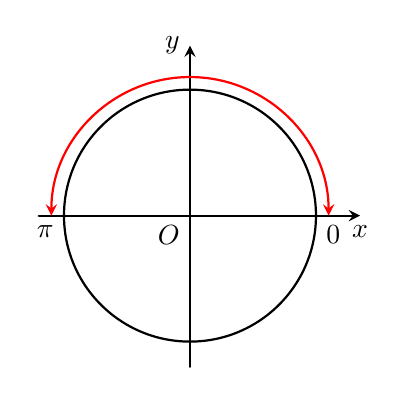
\begin{tikzpicture}[line join=round, line cap=round,>=stealth,thick,scale=0.8]
				\tikzset{label style/.style={font=\footnotesize}}
				\draw[->] (-2.4,0)--(2.7,0) node[below] {$x$};
				\draw[->] (0,-2.4)--(0,2.7) node[left] {$y$};
				\draw (0,0) node [below left] {$O$};
				\draw (2,0) node [below right] {$0$};
				\draw (-2,0) node [below left] {$\pi$};
				\draw (0,0) circle (2);
				\draw[red,<->] (2.2,0) arc (0:180:2.2 cm);
			\end{tikzpicture}
		}	
	}
\end{bt}

\begin{bt}%[Bùi Thanh Cương-TeX11-Lbt-DuAn2.1]%[1D1G1-5]
	Tìm giá trị lớn nhất và giá trị nhỏ nhất của hàm số $y=\sin 2 x+2$ trên $\left[ 0; \dfrac{\pi}{2}\right]$?
	\dapso{
		$\max\limits_{x \in \left[ 0; \tfrac{\pi}{2}\right]} y=3$ khi $x=\dfrac{\pi}{4}$ và $\min\limits_{x \in \left[ 0; \tfrac{\pi}{2}\right]} y=2$ khi $x=0$.
	}
	\loigiai
	{\immini
		{Ta có $x\in \left[ 0; \dfrac{\pi}{2}\right]\Rightarrow 2x\in \left[ 0; \pi\right]$.\\
			Với mọi $2x\in \left[ 0; \pi\right]$ ta có
			\allowdisplaybreaks
			\begin{eqnarray*}
				& & 0\leq \sin 2x\leq 1\\
				&\Leftrightarrow&2\leq \sin 2x+2\leq 3.
			\end{eqnarray*}
			Vậy $\max\limits_{x \in \left[ 0; \tfrac{\pi}{2}\right]} y=3$ khi $x=\dfrac{\pi}{4}$ và $\min\limits_{x \in \left[ 0; \tfrac{\pi}{2}\right]} y=2$ khi $x=0$.
		}
		{
			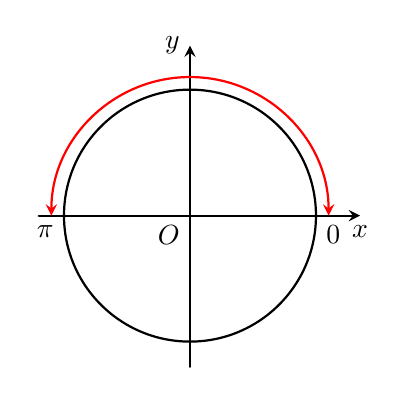
\begin{tikzpicture}[line join=round, line cap=round,>=stealth,thick,scale=0.8]
				\tikzset{label style/.style={font=\footnotesize}}
				\draw[->] (-2.4,0)--(2.7,0) node[below] {$x$};
				\draw[->] (0,-2.4)--(0,2.7) node[left] {$y$};
				\draw (0,0) node [below left] {$O$};
				\draw (2,0) node [below right] {$0$};
				\draw (-2,0) node [below left] {$\pi$};
				\draw (0,0) circle (2);
				\draw[red,<->] (2.2,0) arc (0:180:2.2 cm);
			\end{tikzpicture}
		}
	}
\end{bt}

\begin{bt}%[Bùi Thanh Cương-TeX11-Lbt-DuAn2.1]%[1D1G1-5]
	Tìm giá trị lớn nhất và giá trị nhỏ nhất của hàm số $y=\cos \left(x+\dfrac{\pi}{3}\right)$ trên $[0 ; \pi]$.
	\dapso{
		$\max\limits_{x \in [0 ; \pi]} y=\dfrac{1}{2}$ khi $x=0$ và $\min\limits_{x \in [0 ; \pi]} y=-1$ khi $x=\dfrac{2\pi}{3}$.
	}
	\loigiai
	{\immini
		{Ta có $x\in \left[ 0; \pi\right]\Rightarrow x+\dfrac{\pi}{3}\in \left[ \dfrac{\pi}{3}; \dfrac{4\pi}{3}\right]$.\\
			Do đó: $ -1 \leq \cos \left(x+\dfrac{\pi}{3}\right)\leq \dfrac{1}{2}$.\\
			Vậy $\max\limits_{x \in [0 ; \pi]} y=\dfrac{1}{2}$ khi $x=0$ và $\min\limits_{x \in [0 ; \pi]} y=-1$ khi $x=\dfrac{2\pi}{3}$.
		}
		{
			\begin{tikzpicture}[line join=round, line cap=round,>=stealth,thick,scale=1.4]
				\tikzset{label style/.style={font=\footnotesize}}
				\draw[->] (-1.2,0)--(1.4,0) node[below] {$x$};
				\draw[->] (0,-1.2)--(0,1.3) node[left] {$y$};
				\draw (0,0) circle (1);
				\draw (0,0) node [below left] {$O$};
				\path
				(0,0) coordinate (O)
				($(O) + (60:1.1)$) coordinate (A)
				($(O) + (240:1.1)$) coordinate (B)
				;
				\draw[red,<->] (A) arc (60:240:1.1 cm);
				\draw (O) -- (A) node [right] {\scriptsize $\frac{\pi}{3}$};
				\draw (O) -- (B) node [below] {\scriptsize $\frac{4\pi}{3}$};
				\draw[dashed] (60:1) -- (0.5,0) node [below] {\scriptsize $\frac{1}{2}$};
				\draw[dashed] (240:1) -- (-0.5,0) node [above] {\scriptsize $-\frac{1}{2}$};
			\end{tikzpicture}
		}
	}
\end{bt}

\begin{bt}%[Bùi Thanh Cương-TeX11-Lbt-DuAn2.1]%[1D1G1-5]
	Tìm giá trị lớn nhất và giá trị nhỏ nhất của hàm số $y=\sin \left(2 x+\dfrac{\pi}{4}\right)+\dfrac{1}{2}$ trên $\left[-\dfrac{\pi}{4} ; \dfrac{\pi}{4}\right]$.
	\dapso{
		$\max\limits_{x \in\left[-\tfrac{\pi}{4} ; \tfrac{\pi}{4}\right]} y=\dfrac{3}{2}$ và $\min\limits_{x \in \left[-\tfrac{\pi}{4} ; \tfrac{\pi}{4}\right]} y=\dfrac{1-\sqrt{2}}{2}$.
	}
	\loigiai
	{\immini
		{Ta có $x\in \left[ -\dfrac{\pi}{4} ; \dfrac{\pi}{4}\right]\Rightarrow 2x+\dfrac{\pi}{4}\in \left[ -\dfrac{\pi}{4}; \dfrac{3\pi}{4}\right]$.\\
			Do đó: 
			\allowdisplaybreaks
			\begin{eqnarray*}
				& & -\dfrac{\sqrt{2}}{2}\leq \sin \left(2 x+\dfrac{\pi}{4}\right)\leq 1\\
				&\Rightarrow & \dfrac{1-\sqrt{2}}{2}\leq \sin \left(2 x+\dfrac{\pi}{4}\right)+\dfrac{1}{2}\leq \dfrac{3}{2}.
			\end{eqnarray*}
			Vậy $\max\limits_{x \in\left[-\tfrac{\pi}{4} ; \tfrac{\pi}{4}\right]} y=\dfrac{3}{2}$ và $\min\limits_{x \in \left[-\tfrac{\pi}{4} ; \tfrac{\pi}{4}\right]} y=\dfrac{1-\sqrt{2}}{2}$.
		}
		{
			\begin{tikzpicture}[line join=round, line cap=round,>=stealth,thick,scale=1.4]
				\tikzset{label style/.style={font=\footnotesize}}
				\draw[->] (-1.2,0)--(1.4,0) node[below] {$x$};
				\draw[->] (0,-1.2)--(0,1.3) node[left] {$y$};
				\draw (0,0) circle (1);
				\draw (0,0) node [below left] {$O$};
				\path
				(0,0) coordinate (O)
				($(O) + (-45:1.1)$) coordinate (A)
				($(O) + (135:1.1)$) coordinate (B)
				;
				\draw[red,<->] (A) arc (-45:135:1.1 cm);
				\draw (O) -- (A) node [right] {\scriptsize $-\frac{\pi}{4}$};
				\draw (O) -- (B) node [left] {\scriptsize $\frac{3\pi}{4}$};
				\draw[dashed] (-45:1) -- (0,-0.7) node [left] {\scriptsize $-\frac{\sqrt{2}}{2}$};
				\draw[dashed] (135:1) -- (0,0.7) node [right] {\scriptsize $\frac{\sqrt{2}}{2}$};
			\end{tikzpicture}
		}
	}
\end{bt}

\begin{bt}%[Bùi Thanh Cương-TeX11-Lbt-DuAn2.1]%[1D1G1-5]
	Tìm giá trị lớn nhất và giá trị nhỏ nhất của hàm số $y=\sin^4 x+\cos^4 x$ trên $\left[0 ; \dfrac{\pi}{6}\right]$.
	\dapso{
		$\max\limits_{x \in \left[0 ; \tfrac{\pi}{6}\right]} y=0$ và $\min\limits_{x \in \left[0 ; \tfrac{\pi}{6}\right]} y=-\dfrac{3}{8}$.
	}
	\loigiai
	{Ta có
		\allowdisplaybreaks
		\begin{eqnarray*}
			\sin^4 x+\cos^4 x
			&=& \left(\sin^2 x+\cos^2 x\right)^2-2\sin^2 x\cdot \cos^2 x=1-\dfrac{1}{2}\sin^2 2x\\
			&=&1-\dfrac{1-\cos 4x}{4}= \dfrac{3}{4}+\dfrac{1}{4}\cos 4x.
		\end{eqnarray*}
		Suy ra: $y=\sin^4 x+\cos^4 x-1=\dfrac{1}{4}\cos 4x-\dfrac{1}{4}$.
		\immini
		{ Do $x\in \left[ 0 ; \dfrac{\pi}{6}\right]\Rightarrow 4x \in \left[0; \dfrac{2\pi}{3}\right]$.\\
			Do đó: 
			\allowdisplaybreaks
			\begin{eqnarray*}
				& & -\dfrac{1}{2}\leq\cos 4x \leq 1\\
				&\Leftrightarrow& -\dfrac{1}{8}\leq \dfrac{1}{4}\cos 4x \leq \dfrac{1}{4}\\
				&\Leftrightarrow& -\dfrac{3}{8}\leq \dfrac{1}{4}\cos 4x-\dfrac{1}{4} \leq 0.
			\end{eqnarray*}
			Vậy $\max\limits_{x \in \left[0 ; \tfrac{\pi}{6}\right]} y=0$ và $\min\limits_{x \in \left[0 ; \tfrac{\pi}{6}\right]} y=-\dfrac{3}{8}$.
		}
		{
			\begin{tikzpicture}[line join=round, line cap=round,>=stealth,thick,scale=1.4]
				\tikzset{label style/.style={font=\footnotesize}}
				\draw[->] (-1.2,0)--(1.4,0) node[below] {$x$};
				\draw[->] (0,-1.2)--(0,1.3) node[left] {$y$};
				\draw (0,0) circle (1);
				\draw (0,0) node [below left] {$O$};
				\path
				(0,0) coordinate (O)
				($(O) + (0:1.1)$) coordinate (A)
				($(O) + (120:1.1)$) coordinate (B)
				;
				\draw[red,<->] (A) arc (0:120:1.1 cm);
				\draw (O) -- (A) node [below] {\scriptsize $0$};
				\draw (O) -- (B) node [above] {\scriptsize $\frac{2\pi}{3}$};
				\draw[dashed] (120:1) -- (-0.5,0) node [below] {\scriptsize $\frac{1}{2}$};
			\end{tikzpicture}
		}
		
	}
\end{bt}

\begin{bt}%[Bùi Thanh Cương-TeX11-Lbt-DuAn2.1]%[1D1G1-5]
	Tìm giá trị lớn nhất và giá trị nhỏ nhất của hàm số $y=\sin^6 x+\cos^6 x$  trên $\left[-\dfrac{\pi}{2} ; \dfrac{\pi}{2}\right]$.
	\dapso{
		$\max\limits_{x \in \left[-\tfrac{\pi}{2} ; \tfrac{\pi}{2}\right]} y=1$ và $\min\limits_{x \in \left[-\tfrac{\pi}{2} ; \tfrac{\pi}{2}\right]} y=\dfrac{1}{4}$.
	}
	\loigiai{Ta có
		\allowdisplaybreaks
		\begin{eqnarray*}
			\sin^6 x+\cos^6 x
			&=& \left(\sin^2 x+\cos^2 x\right)^3-3\sin^2 x\cdot \cos^2 x\left(\sin^2 x+\cos^2 x \right)=1-\dfrac{3}{4}\sin^2 2x\\
			&=&1-\dfrac{3}{4}\cdot \dfrac{1-\cos 4x}{2}= \dfrac{5}{8}+\dfrac{3}{8}\cos 4x.
		\end{eqnarray*}
		Suy ra: $y=\sin^6 x+\cos^6 x = \dfrac{5}{8}+\dfrac{3}{8}\cos 4x$.\\
		Do $x\in \left[-\dfrac{\pi}{2} ; \dfrac{\pi}{2} \right]\Rightarrow 4x \in \left[-2\pi ; 2\pi\right]$  nên 
		\allowdisplaybreaks
		\begin{eqnarray*}
			& & -1\leq\cos 4x \leq 1\\
			&\Leftrightarrow& -\dfrac{3}{8}\leq \dfrac{3}{8}\cos 4x \leq \dfrac{3}{8}\\
			&\Leftrightarrow& \dfrac{1}{4}\leq \dfrac{5}{8}+ \dfrac{3}{8}\cos 4x \leq 1.
		\end{eqnarray*}
		Vậy $\max\limits_{x \in \left[-\tfrac{\pi}{2} ; \tfrac{\pi}{2}\right]} y=1$ và $\min\limits_{x \in \left[-\tfrac{\pi}{2} ; \tfrac{\pi}{2}\right]} y=\dfrac{1}{4}$.
	}
\end{bt}

\begin{bt}%[Bùi Thanh Cương-TeX11-Lbt-DuAn2.1]%[1D1G1-5]
	Tìm giá trị lớn nhất và giá trị nhỏ nhất của hàm số $y=\sqrt{3} \sin 2 x+2 \cos^2 x+3$ trên $\left[-\dfrac{5 \pi}{6}; \dfrac{\pi}{4}\right]$.
	\dapso{
		$\max\limits_{x \in \left[-\tfrac{5 \pi}{6}; \tfrac{\pi}{4}\right]} y=6$ và $\min\limits_{x \in \left[-\tfrac{5 \pi}{6}; \tfrac{\pi}{4}\right]} y=2$.
	}
	\loigiai
	{Ta có
		\allowdisplaybreaks
		\begin{eqnarray*}
			y
			&=& \sqrt{3} \sin 2 x+2 \cos^2 x+3\\
			&=&\sqrt{3} \sin 2 x+2\cdot\dfrac{1+\cos 2x}{2}+3\\
			&=& \sqrt{3} \sin 2 x+\cos 2x+4=2\sin \left(2x+\dfrac{\pi}{6}\right)+4.
		\end{eqnarray*}
		Do $x\in \left[ -\dfrac{5 \pi}{6}; \dfrac{\pi}{4}\right]\Rightarrow 2x \in \left[-\dfrac{5 \pi}{3}; \dfrac{\pi}{2}\right] \Rightarrow 2x +\dfrac{\pi}{6}\in \left[-\dfrac{3\pi}{2}; \dfrac{2\pi}{3}\right]$ .\\
		Do đó: 
		\allowdisplaybreaks
		\begin{eqnarray*}
			& & -1\leq \sin \left(2x+\dfrac{\pi}{6}\right) \leq 1\\
			&\Leftrightarrow& -2\leq 2\sin \left(2x+\dfrac{\pi}{6}\right) \leq 2\\
			&\Leftrightarrow& 2\leq 2\sin \left(2x+\dfrac{\pi}{6}\right)+4 \leq 6.
		\end{eqnarray*}
		Vậy $\max\limits_{x \in \left[-\tfrac{5 \pi}{6}; \tfrac{\pi}{4}\right]} y=6$ và $\min\limits_{x \in \left[-\tfrac{5 \pi}{6}; \tfrac{\pi}{4}\right]} y=2$.
	}
\end{bt}

\begin{bt}%[Bùi Thanh Cương-TeX11-Lbt-DuAn2.1]%[1D1G1-5]
	Tìm giá trị lớn nhất và giá trị nhỏ nhất của hàm số $y=\sin 2 x+\cos 2 x+3$ trên $\left[-\dfrac{\pi}{4} ; \dfrac{\pi}{4}\right]$.
	\dapso{
		$\max\limits_{x \in \left[-\tfrac{\pi}{4} ; \tfrac{\pi}{4}\right]} y=3+\sqrt{2}$ và $\min\limits_{x \in \left[-\tfrac{\pi}{4} ; \tfrac{\pi}{4}\right]} y=2$.
	}
	\loigiai
	{Ta có $ y	= \sin 2 x+\cos 2 x+3= \sqrt{2}\sin \left(2x+\dfrac{\pi}{4}\right)+3$.
		\immini
		{ Do $x\in \left[-\dfrac{\pi}{4} ; \dfrac{\pi}{4}\right]\Rightarrow 2x \in \left[-\dfrac{\pi}{2} ; \dfrac{\pi}{2}\right] \Rightarrow 2x +\dfrac{\pi}{4}\in \left[-\dfrac{\pi}{4}; \dfrac{3\pi}{4}\right]$ .\\
			Do đó: 
			\allowdisplaybreaks
			\begin{eqnarray*}
				& & -\dfrac{\sqrt{2}}{2}\leq\sin \left(2x+\dfrac{\pi}{4}\right) \leq 1\\
				&\Leftrightarrow& -1\leq  \sqrt{2} \sin \left(2x+\dfrac{\pi}{4}\right)\leq \sqrt{2}\\
				&\Leftrightarrow& 2\leq \sqrt{2}\sin \left(2x+\dfrac{\pi}{4}\right)+3 \leq 3+\sqrt{2}.
			\end{eqnarray*}
			Vậy $\max\limits_{x \in \left[-\tfrac{\pi}{4} ; \tfrac{\pi}{4}\right]} y=3+\sqrt{2}$ và $\min\limits_{x \in \left[-\tfrac{\pi}{4} ; \tfrac{\pi}{4}\right]} y=2$.
		}
		{
			\begin{tikzpicture}[line join=round, line cap=round,>=stealth,thick,scale=1.6]
				\tikzset{label style/.style={font=\footnotesize}}
				\draw[->] (-1.2,0)--(1.3,0) node[below] {$x$};
				\draw[->] (0,-1.2)--(0,1.3) node[left] {$y$};
				\draw (0,0) circle (1);
				\draw (0,0) node [below left] {$O$};
				\path
				(0,0) coordinate (O)
				($(O) + (-45:1.1)$) coordinate (A)
				($(O) + (135:1.1)$) coordinate (B)
				;
				\draw[red,<->] (A) arc (-45:135:1.1 cm);
				\draw (O) -- (A) node [right] {\scriptsize $-\frac{\pi}{4}$};
				\draw (O) -- (B) node [left] {\scriptsize $\frac{3\pi}{4}$};
				\draw[dashed] (135:1) -- (0,0.7) node [right=-3pt] {\scriptsize $\frac{\sqrt{2}}{2}$};
				\draw[dashed] (-45:1) -- (0,-0.7) node [left=-1pt] {\scriptsize $-\frac{\sqrt{2}}{2}$};
			\end{tikzpicture}
		}
		
	}
\end{bt}


%%%%%%%%% Thầy Danh Trần %%%%%%%
\begin{bt}%[THPT chuyên Phan Bội Châu $-$ Nghệ An]%[Danh Trần - DA2.1]%[1D1G1-5]
	Giá trị lớn nhất của hàm số $y=\sin^9 x+\cos^{12}x$ bằng
	\choice
	{$2$}
	{\True $1$}
	{$0{,}5$}
	{$1{,}5$}
	\loigiai
	{
		Ta có $\sin^9 x\le \sin^2 x$, $\cos^{12}x\le \cos^2x$ do $\sin x,\,\cos x\in[-1;1]$.\\
		Do đó $y\le \sin^2 x+\cos ^2x=1$, nên giá trị lớn nhất của hàm số là $y=1$.\\
		Đẳng thức xảy ra khi $\sin x=0$ hoặc $\cos x=0$, từ đó suy ra $x=\dfrac{k\pi}{2}$, $k\in\mathbb{Z}$.
	}
\end{bt}
\begin{bt}%[Tạp chí Toán học \& Tuổi trẻ, số 489]%[Danh Trần - DA2.1]%[1D1G1-5]
	Số giờ có ánh sáng của một thành phố $X$ ở vĩ độ $40^\circ$ Bắc trong ngày thứ $t$ của một năm không nhuận được cho bởi hàm số $d(t)=3\sin\left[\dfrac{\pi}{182}(t-80)\right]+12$, $t\in\mathbb{Z}$ và $0<t\le 365$. Vào ngày nào trong năm thì thành phố $X$ có nhiều giờ ánh sáng nhất?
	\choice
	{$262$}
	{$353$}
	{$80$}
	{\True $171$}
	\loigiai
	{
		Ta có $d(t)=3\sin\left[\dfrac{\pi}{182}(t-80)\right]+12\le 3+12=15$.\\
		Nên thành phố $X$ có nhiều giờ ánh sáng nhất thì $d(t)=15$.\\
		Đẳng thức xảy ra khi $\sin\left[\dfrac{\pi}{182}(t-80)\right]=1\Leftrightarrow \dfrac{\pi}{182}(t-80)=\dfrac{\pi}{2}+k2\pi$, $k\in\mathbb{Z}$
		\[\Leftrightarrow \dfrac{t-80}{182}=\dfrac{4k+1}{2}\Leftrightarrow t=91(4k+1)+80=364k+171.\]
		Do $0<t\le 365$ nên $k=0$, khi đó với $t=171$ thì thành phố $X$ có nhiều giờ ánh sáng nhất.
	}
\end{bt}
\begin{bt}%[THPT Minh Châu $-$ Hưng Yên, 2019]%[Danh Trần - DA2.1]%[1D1K1-5]
	Hằng ngày, mực nước của con kênh lên xuống theo thủy triều. Độ cao $h$ (m) của mực nước trong kênh tính theo thời gian $t$ (h) được cho bởi công thức $h=3\cos\left(\dfrac{\pi t}{6}+\dfrac{\pi}{3}\right)+12$. Khi nào mực nước của kênh là cao nhất với thời gian ngắn nhất?
	\choice
	{$t=22$ (h)}
	{$t=15$ (h)}
	{$t=14$ (h)}
	{\True $t=10$ (h)}
	\loigiai
	{
		Ta có $h=3\cos\left(\dfrac{\pi t}{6}+\dfrac{\pi}{3}\right)+12\le 3+12=15$ nên mực nước của kênh cao nhất là $h=15$ (m).\\
		Đẳng thức xảy ra khi $\cos\left(\dfrac{\pi t}{6}+\dfrac{\pi}{3}\right)=1\Leftrightarrow \dfrac{\pi t}{6}+\dfrac{\pi}{3}=k2\pi\Leftrightarrow t=12k-2$, $k\in\mathbb{Z}$.\\
		Do thời gian ngắn nhất và dương nên $k=1$, khi đó $t=10$ (h).
	}
\end{bt}